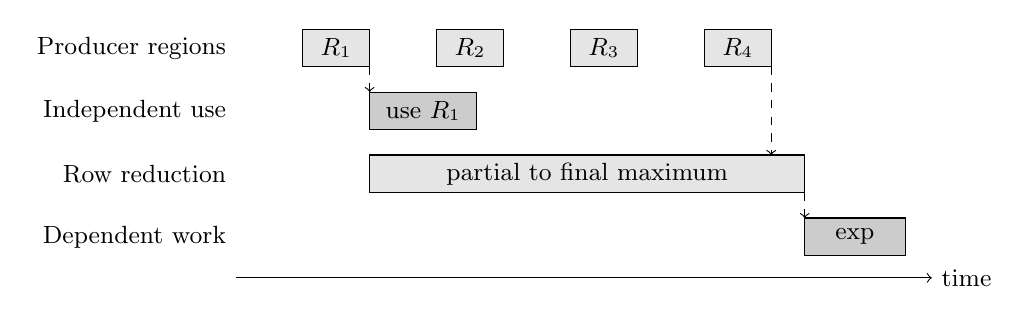
\begin{tikzpicture}[x=0.85cm,y=0.8cm, every node/.style={font=\small}]
 \node[anchor=east] at (0,3) {Producer regions};
 \node[anchor=east] at (0,2) {Independent use};
 \node[anchor=east] at (0,1) {Row reduction};
 \node[anchor=east] at (0,0) {Dependent work};
 \draw[->] (0,-0.65)--(10.4,-0.65) node[right] {time};
 \foreach \x/\n in {1/1,3/2,5/3,7/4} {
   \draw[fill=black!10] (\x,2.7) rectangle (\x+1,3.3);
   \node at (\x+0.5,3) {$R_{\n}$};
 }
 \draw[fill=black!20] (2,1.7) rectangle (3.6,2.3);
 \node at (2.8,2) {use $R_1$};
 \draw[->,dashed] (2,2.7)--(2,2.3);
 \draw[fill=black!10] (2,0.7) rectangle (8.5,1.3);
 \node at (5.25,1) {partial to final maximum};
 \draw[->,dashed] (8,2.7)--(8,1.3);
 \draw[fill=black!20] (8.5,-0.3) rectangle (10,0.3);
 \node at (9.25,0) {exp};
 \draw[->,dashed] (8.5,0.7)--(8.5,0.3);
\end{tikzpicture}
